\newthought{\textbf{Rauzatinur Syah - 2020903430039 - TRKJ 3B}}


\newday{\textbf{1 - 2 Desember 2022} - Instalasi dan Konfigurasi Hadoop}
\begin{enumerate}
\item Kendala dan Solusi\\
% jelaskan kendala dan penyebab yang dialami saat mengikuti praktikum serta solusi atau langkah-langkah yang telah dilakukan
\begin{enumerate}
\item Kendala
\begin{itemize}
\item terdapat kendala pada instalasi hadoop pada pengecekanan versi hadoop yang berfungsi untuk menverifikasi instalasi hadoop
\item terdapat kendala saat menjalanakn format HDFS dan hadoop service
\end{itemize}
\item Solusi \\
\begin{itemize}
\item melakukan pengecekan pada file hadoop-env.sh
\item melakuka  pengecekan pada file core-site.xml, hdfs-site.xml, mapred-site.xml, yarn-site.xml
\end{itemize}
\end{enumerate}

\item Kesimpulan\\
% berikan kesimpulan dari praktikum yang telah dikerjkan
adapun kesimpulan yang diperoleh yaitu instalasi dan konfigurasi hadoop berhasil 
\end{enumerate}

\begin{figure}[!ht]
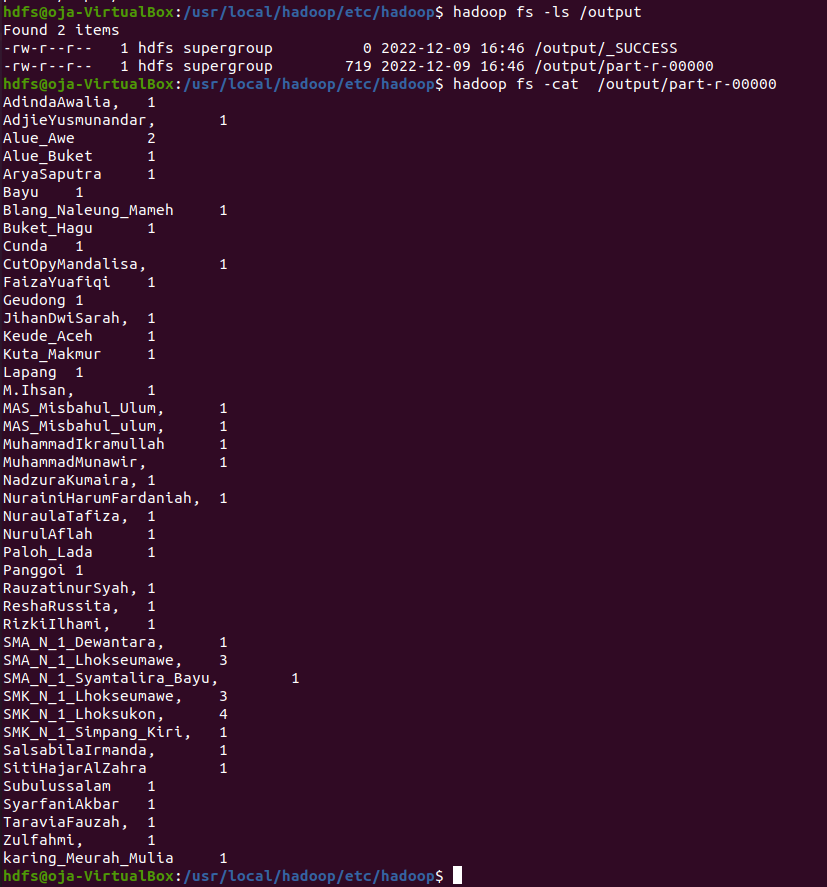
\includegraphics[width=\textwidth]{RauzatinurSyah/dataHadoop}
\caption{hasil program WordCount hadoop}
\label{gam:Hasil}
\end{figure}

\newday{\textbf{8 Desember 2022} - WordCount bawaan Hadoop}
\begin{enumerate}
\item Kendala dan Solusi\\
% jelaskan kendala dan penyebab yang dialami saat mengikuti praktikum serta solusi atau langkah-langkah yang telah dilakukan
pada pratikum Program WordCount bawaan hadoop tidak ada kendala pada praktikum yang dilakukan
\item Kesimpulan\\
% berikan kesimpulan dari praktikum yang telah dikerjkan
berhasil menjalanakan program wordCount bawan hadoop
\end{enumerate}


\begin{figure}[!ht]
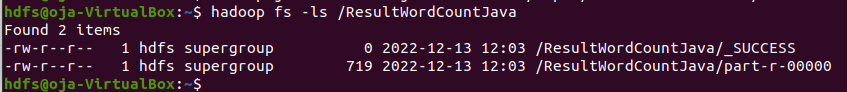
\includegraphics[width=\textwidth]{RauzatinurSyah/datahadoopjava no 9}
\caption{hasil program WordCount java no.9}
\label{gam:hasil program}
\end{figure}

\begin{figure}[!ht]
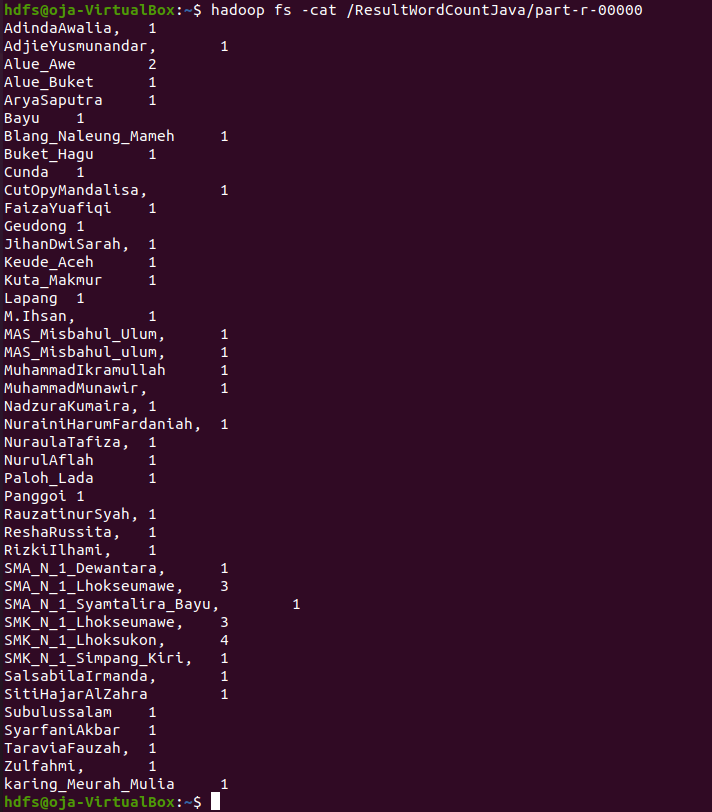
\includegraphics[width=\textwidth]{RauzatinurSyah/datahadoopjava no 10}
\caption{hasil program WordCount java no.10}
\label{gam:hasil program}
\end{figure}

\newday{\textbf{9 Desember 2022} - WordCount dengan Java}
\begin{enumerate}
\item Kendala dan Solusi \\
% jelaskan kendala dan penyebab yang dialami saat mengikuti praktikum serta solusi atau langkah-langkah yang telah dilakukan
pada praktikum WordCount dengan java
\begin{enumerate}
\item kendala: \\
terdapat kendala pada perintah menjalankan program dengan perintah"hadoop jar WordCount.jar WordCount /input/data/WordCount.txt /ResultWourdCountJava"
\item solusi: \\
menjalankan hadoop service dengan perintah "start-all.sh" dikarnakan terdapat kesalahan yang dilakukan yaitu tidak menjalankan hadoop service
\end{enumerate}
\item Kesimpulan\\
% berikan kesimpulan dari praktikum yang telah dikerjkan
adapun kesimpulan yang diperoleh yaitu berhasil menjalankan programa tersebut 
\end{enumerate}
